\chapter{Algorithm Design and Implementation} \label{ch:Alg_Design}

\section{UKF Formulation} \label{sec:ukf_formulation}

In this section, we develop a formulation of the Unscented Kalman Filter for estimating the state of a quadcopter. We begin with the two overarching phases of the algorithm, prediction and correction. Then we develop a kinematic process model which describes the vehicle's motion over time. After this, we develop an observation model which describes the relationship between the vehicle's state and the vehicle's sensor readings. Finally, we explore noise models which describe the Gaussian noise present in both the process and observation models.

\subsection{Prediction Step}

We begin by defining the following quantities:
%
\begin{align} \label{eq:state_vars}
\mathbf{p} &= \left\lbrace x,\ y,\ z \right\rbrace ^{T} \\
\mathbf{q} &= \left\lbrace q_{x},\ q_{y},\ q_{z},\ q_{w} \right\rbrace ^{T} \label{eq:quat_convention} \\
\mathbf{v} &= \left\lbrace \dot{x},\ \dot{y},\ \dot{z} \right\rbrace ^{T} \\
\bm{\Omega} &= \left\lbrace \omega_{x},\ \omega_{y},\ \omega_{z} \right\rbrace ^{T} \\
\mathbf{a} &= \left\lbrace \ddot{x},\ \ddot{y},\ \ddot{z} \right\rbrace ^{T}
\end{align}
%
The vectors $\mathbf{p}$, $\mathbf{v}$, and $\mathbf{a}$ represent the vehicle's position, velocity, and acceleration, respectively. The quaternion\footnote{All quaternion are represented here according to the convention used in equation~\ref{eq:quat_convention}, where $q_{w}$ is the scalar component and is always placed in the last position. This convention was chosen to maintain consistency with the Eigen library's internal representation of quaternions.} $\mathbf{q}$ represents the vehicle's orientation, and the vector $\bm{\Omega}$ represents the vehicle's angular rates. We now define the state vector $\mathbf{x}$ as
%
\begin{equation}
\mathbf{x} = 
\Big\{
    \mathbf{p}^{T},\
    \mathbf{q}^{T},\
    \mathbf{v}^{T},\
    \bm{\Omega}^{T},\
    \mathbf{a}^{T}
\Big\} ^{T}
\end{equation}
%
and let $n = 16$ represent the number of state variables.

Let $\mathbf{P} \in \mathbb{R}^{n \times n}$ be the covariance matrix associated with the state $\mathbf{x}$. A set of $2n + 1$ sigma points is then derived from $\mathbf{x}$ and $\mathbf{P}$ as
%
\begin{align}
\bm{\chi}^{0}_{k-1 | k-1} &= \mathbf{x}_{k-1 | k-1} \nonumber\\
\bm{\chi}^{i}_{k-1 | k-1} &= \mathbf{x}_{k-1 | k-1} + \left( \sqrt{\left( n + \lambda \right) \mathbf{P}_{k-1 | k-1}} \right)_{i}, &&i = 1,\ \dots,\ n \\
\bm{\chi}^{i}_{k-1 | k-1} &= \mathbf{x}_{k-1 | k-1} - \left( \sqrt{\left( n + \lambda \right) \mathbf{P}_{k-1 | k-1}} \right)_{i-n}, &&i = n+1,\ \dots,\ 2n \nonumber
\end{align}
%
where $\bm{\chi}^{i}$ is the $i$-th sigma point and $\left( \sqrt{\left( n + \lambda \right) \mathbf{P}_{k-1 | k-1}} \right)_{i}$ is the $i$-th column of the square root matrix $\sqrt{\left( n + \lambda \right) \mathbf{P}_{k-1 | k-1}}$. The square root matrix $\mathbf{A}$ of a matrix $\mathbf{B}$ is defined here as
%
\begin{equation}
\mathbf{A} \mathbf{A}^{T} = \mathbf{B}
\end{equation}
%
and is evaluated using Cholesky decomposition\footnote{\url{https://en.wikipedia.org/wiki/Cholesky_decomposition\#The_Cholesky_algorithm}} for computational efficiency.

To predict the next state, the sigma points are propagated through the nonlinear process function $f$ (defined in Section~\ref{Process_Model}):
%
\begin{equation}
\bm{\chi}^{i}_{k | k-1} = f \left( \bm{\chi}^{i}_{k-1 | k-1} \right), \quad i = 0,\ \dots,\ 2n
\end{equation}
%
These transformed sigma points are then used to determine the predicted state $\hat{\mathbf{x}}_{k | k-1}$ and its associated covariance $\mathbf{P}_{k | k-1}$ as
%
\begin{align}
\hat{\mathbf{x}}_{k | k-1} &= \sum^{2n}_{i=0} W^{i}_{s} \bm{\chi}^{i}_{k | k-1} \label{eq:pred_state} \\
\mathbf{P}_{k | k-1} &= \left( \sum^{2n}_{i=0} W^{i}_{c} \left( \bm{\chi}^{i}_{k | k-1} - \hat{\mathbf{x}}_{k | k-1} \right) \left( \bm{\chi}^{i}_{k | k-1} - \hat{\mathbf{x}}_{k | k-1} \right)^{T} \right) + \mathbf{Q}  \label{eq:pred_cov}
\end{align}
%
where $\mathbf{Q}$ is the process noise covariance matrix (defined in Section~\ref{sec:Q_Matrix}).

The state weights $W_{s}$ and covariance weights $W_{c}$ used in equations~\ref{eq:pred_state} and \ref{eq:pred_cov} (and later in equations~\ref{eq:zHat}, \ref{eq:P_zz}, and \ref{eq:P_xz}) are defined as
%
\begin{align}
W^{0}_{s} &= \dfrac{\lambda}{n + \lambda} \nonumber \\
W^{0}_{c} &= \dfrac{\lambda}{n + \lambda} + \left( 1 - \alpha^{2} + \beta \right) \\
W^{i}_{s} &= W^{i}_{c} = \dfrac{1}{2 \left(n + \lambda \right)}, \quad i = 1,\ \dots,\ 2n \nonumber
\end{align}
%
where the constants $\alpha$, $\beta$, $\kappa$, and $\lambda$ are defined as
%
\begin{align}
\alpha &= 0.75 \\
\beta &= 2 \\
\kappa &= 0 \\
\lambda &= \alpha^{2} \left( n + \kappa \right) - n = -7
\end{align}
%
These constants control the spread of the sigma points chosen within the filter. According to Wan et al.\ in \cite{Wan2000}, setting $\beta = 2$ is optimal for a Gaussian state distribution, and $\kappa$ is commonly set to zero. The value of $\alpha$ is usually small and positive. Here, we chose $\alpha$ by trial and error after observing the rate at which the filter converged in a number of preliminary experiments. We found that choosing $0 < \alpha \leq 0.5$ made the filter slow to converge. The filter's estimates would lag behind the pose sensor's readings by an interval that was sometimes several seconds in length and, in steady state, would undershoot the pose sensor. Conversely, choosing $\alpha \geq 1$ caused the filter to diverge. At $\alpha \approx 0.75$, the filter had no distinguishable lag and was highly stable.

\subsection{Correction Step}

Given the belief defined by $\mathbf{x}_{k | k-1}$ and $\mathbf{P}_{k | k-1}$, we compute $2n + 1$ sigma points again as
%
\begin{align}
\bm{\chi}^{0}_{k | k-1} &= \mathbf{x}_{k | k-1} & \nonumber\\
\bm{\chi}^{i}_{k | k-1} &= \mathbf{x}_{k | k-1} + \left( \sqrt{\left( n + \lambda \right) \mathbf{P}_{k | k-1}} \right)_{i}, &&i = 1,\ \dots,\ n \\
\bm{\chi}^{i}_{k | k-1} &= \mathbf{x}_{k | k-1} - \left( \sqrt{\left( n + \lambda \right) \mathbf{P}_{k | k-1}} \right)_{i-n}, &&i = n+1,\ \dots,\ 2n \nonumber
\end{align}
%
Next, the sigma points are projected into the sensor space through the observation function $h$ (defined in Section~\ref{Observation_Model}):
%
\begin{equation}
\bm{\gamma}^{i}_{k} = h \left( \bm{\chi}^{i}_{k | k-1} \right), \quad i = 0,\ \dots,\ 2n
\end{equation}

Let $m = 7$ represent the number of measurements taken from each PTAM message. Each of these messages is mathematically interpreted as an $m$-dimensional measurement vector $\mathbf{z}_{k}$ of the form
%
\begin{equation}
\mathbf{z}_{k} = \left\lbrace x,\ y,\ z,\ q_{x},\ q_{y},\ q_{z},\ q_{w} \right\rbrace ^{T} _{\text{meas.}} 
\end{equation}
%
The predicted measurement vector $\hat{\mathbf{z}}_{k}$ and measurement noise covariance $\mathbf{P}_{zz}$ are then computed as
%
\begin{align}
\hat{\mathbf{z}}_{k} &= \sum^{2n}_{i=0} W^{i}_{s} \bm{\gamma}^{i}_{k} \label{eq:zHat} \\
\mathbf{P}_{zz} &= \left( \sum^{2n}_{i=0} W^{i}_{c} \left( \bm{\gamma}^{i}_{k} - \hat{\mathbf{z}}_{k} \right) \left( \bm{\gamma}^{i}_{k} - \hat{\mathbf{z}}_{k} \right)^{T} \right) + \mathbf{R} \label{eq:P_zz}
\end{align}
%
where $\mathbf{R}$ is the measurement noise covariance matrix (defined in Section~\ref{sec:R_Matrix}). The state-measurement cross-covariance $\mathbf{P}_{xz}$ is then defined as
%
\begin{equation} \label{eq:P_xz}
\mathbf{P}_{xz} = \sum^{2n}_{i=0} W^{i}_{c} \left( \bm{\chi}^{i}_{k | k-1} - \hat{\mathbf{x}}_{k | k-1} \right) \left( \bm{\gamma}^{i}_{k} - \hat{\mathbf{z}}_{k} \right)^{T}
\end{equation}
%
Next, we compute the Kalman gain $\mathbf{K}_{k}$ per the definition
%
\begin{equation}
\mathbf{K}_{k} = \mathbf{P}_{xz} \mathbf{P}^{\,-1}_{zz}
\end{equation}
%
The corrected state $\hat{\mathbf{x}}_{k | k}$ is the sum of the predicted state and the innovation, weighted by $\mathbf{K}_{k}$:
%
\begin{equation}
\hat{\mathbf{x}}_{k | k} = \hat{\mathbf{x}}_{k | k-1} + \mathbf{K}_{k} \left( \hat{\mathbf{z}}_{k} - \mathbf{z}_{k} \right)
\end{equation}
%
The corrected covariance $\mathbf{P}_{k | k}$ is the difference between the predicted state covariance $\mathbf{P}_{k | k-1}$ and the predicted measurement covariance, weighted by the Kalman gain:
%
\begin{equation}
\mathbf{P}_{k | k} = \mathbf{P}_{k | k-1} - \mathbf{K}_{k} \mathbf{P}_{zz} \mathbf{K}_{k}^{T}
\end{equation}

\subsection{Process Model} \label{Process_Model}

To propagate the vehicle's state forward in time, we perform a number of integration operations on the linear accelerations and angular rates measured by the IMU. To determine the orientation of the vehicle at some time $k$, we integrate the measured angular rate vector $\bm{\Omega}_{\text{meas.}}$ per the relationship given in \cite{Stevens2015},
%
\begin{equation} \label{eq:proc_quat}
\mathbf{q}_{k} = \mathbf{q}_{k-1} + \frac{1}{2} \mathbf{\Theta} \left( \bm{\Omega}_{k} \right) \mathbf{q}_{k-1} \Delta t
\end{equation}
%
where $\mathbf{\Theta} \left( \bm{\Omega}_{k} \right) \in \mathbb{R}^{4 \times 4}$ is the angular rate integration matrix defined by
%
\begin{equation}
\mathbf{\Theta} \left( \bm{\Omega}_{k} \right) =
\begin{bmatrix}
0 & \omega_{z} & -\omega_{y} & \omega_{x} \\
-\omega_{z} & 0 & \omega_{x} & \omega_{y} \\
\omega_{y} & -\omega_{x} & 0 & \omega_{z} \\
-\omega_{x} & -\omega_{y} & -\omega_{z} & 0
\end{bmatrix}
\end{equation}
%
and the vehicle's current angular velocity vector is measured directly by the gyroscope:
%
\begin{equation} \label{eq:proc_ang_vel}
\bm{\Omega}_{k} = \bm{\Omega}_{\text{meas.}}
\end{equation}

To calculate the vehicle's current acceleration, we first subtract gravity from the measured acceleration vector $\mathbf{a}_{\text{meas.}}$ and then rotate the difference into the inertial frame:
%
\begin{equation} \label{eq:proc_acc}
\mathbf{a}_{k} = R^{g}_{b,\ k-1} \left( \mathbf{a}_{\text{meas.}} - \mathbf{g} \right)
\end{equation}
%
Here $R^{g}_{b,\ k-1}$ is the rotation matrix representation of the previous orientation quaternion $\mathbf{q}_{k-1}$ and $\mathbf{g}$ is the vector representation of gravity in the global frame. For a given quaternion $\mathbf{q}$, the rotation matrix $R^{g}_{b}$ would be
%
\begin{equation}
R^{g}_{b} =
\begin{bmatrix}[1.5]
    1 - 2 q_{y}^2 - 2 q_{z}^2 & 2 q_{x} q_{y} - 2 q_{z} q_{w} & 2 q_{x} q_{z} + 2 q_{y} q_{w} \\
    2 q_{x} q_{y} + 2 q_{z} q_{w} & 1 - 2 q_{x}^2 - 2 q_{z}^2 & 2 q_{y} q_{z} - 2 q_{x} q_{w} \\
    2 q_{x} q_{z} - 2 q_{y} q_{w} & 2 q_{y} q_{z} + 2 q_{x} q_{w} & 1 - 2 q_{x}^2 - 2 q_{y}^2
\end{bmatrix}
\end{equation}

With the vehicle's current acceleration known, we can compute the current velocity of the vehicle by integrating the vehicle's average acceleration between the current and previous time steps:
%
\begin{equation} \label{eq:proc_vel}
\mathbf{v}_{k} = \mathbf{v}_{k-1} + \frac{1}{2} \left( \mathbf{a}_{k} + \mathbf{a}_{k-1} \right) \Delta t
\end{equation}
%
Similarly, we compute the vehicle's current position using the vehicle's average velocity:
%
\begin{equation} \label{eq:proc_pos}
\mathbf{p}_{k} = \mathbf{p}_{k-1} + \frac{1}{2} \left( \mathbf{v}_{k} + \mathbf{v}_{k-1} \right) \Delta t
\end{equation}

Together, equations~\ref{eq:proc_quat}, \ref{eq:proc_ang_vel}, \ref{eq:proc_acc}, \ref{eq:proc_vel}, and \ref{eq:proc_pos} constitute the nonlinear process function $f$:
%
\begin{equation}
f \left( \mathbf{x}_{k-1 | k-1} \right) = 
\begin{Bmatrix}[1.5]
   \mathbf{p}_{k-1} + \frac{1}{2} \left( \mathbf{v}_{k} + \mathbf{v}_{k-1} \right) \Delta t \\
   \mathbf{q}_{k-1} + \frac{1}{2} \mathbf{\Theta} \left( \bm{\Omega}_{k} \right) \mathbf{q}_{k-1} \Delta t \\
   \mathbf{v}_{k-1} + \frac{1}{2} \left( \mathbf{a}_{k} + \mathbf{a}_{k-1} \right) \Delta t \\
   \bm{\Omega}_{\text{meas.}} \\
   R^{g}_{b,\ k-1} \left( \mathbf{a}_{\text{meas.}} - \mathbf{g} \right)
\end{Bmatrix}
\end{equation}

For purposes of noise modeling, the process function $f$ is modeled according to the relationship
%
\begin{equation}
\mathbf{x}_{k | k-1} = f \left( \mathbf{x}_{k-1 | k-1},\ \bm{\delta}_{k} \right)
\end{equation}
%
where $\bm{\delta}_{k} \sim \mathcal{N} \left( 0,\ \mathbf{Q} \right)$ is additive Gaussian-distributed process noise, assumed to have zero mean and covariance $\mathbf{Q}$ (explored further in Section~\ref{sec:Q_Matrix}).


\subsection{Observation Model} \label{Observation_Model}

Before presenting the observation function $h$, we will first explore several corrective measures employed to improve the numerical stability of the filter. The first of these is an algorithmic approach to quaternion continuity checking. The second is a derived measurement of the vehicle's velocity designed to prevent drift in the absence of direct velocity measurements.

\subsubsection{Quaternion Continuity Correction}

A defect was discovered in the ROS implementation of PTAM during preliminary testing. PTAM's quaternion estimates switch sign without warning after the camera rotates approximately 270 degrees, clockwise or counterclockwise. This aberrant behavior was provoked predictably in dozens of early tests in multiple testing areas, precluding the possibility of a one-off mapping error caused by a particular environment.

Quaternions are defined mathematically such that any quaternion $\mathbf{q}$ and its negative, $- \mathbf{q}$, encode precisely the same \textit{orientation}, but opposite \textit{rotations}. If $\mathbf{q}$ encodes a clockwise rotation of 90 degrees about the $z$-axis, $- \mathbf{q}$ will encode a counterclockwise 270-degree rotation about the same axis. The final orientation is the same in either case, but the two quaternions imply rotations in opposite directions. This has major implications for motion tracking. For example, when estimating the orientation of a vehicle moving in the $xy$-plane, such a sign flip would be visualized as an instantaneous 360-degree rotation about the $z$-axis, implying a massive angular acceleration that never took place. 

A simple way to detect this type of errant behavior is to check, upon receipt of each new quaternion $\mathbf{q}_{k}$, whether $- \mathbf{q}_{k}$ implies a smaller rotation from the previous quaternion $\mathbf{q}_{k-1}$. Given that PTAM produces pose estimates at a rate of about 20~Hz, we assume only small-angle rotations between pose estimates. Thus, the smaller of the two rotations should always come from the correct quaternion. We can compare the relative magnitude of each possible rotation by taking the norm of the ``delta-quaternions'' $\mathbf{q}_{k-1} - \mathbf{q}_{k}$ and $\mathbf{q}_{k-1} - \left( - \mathbf{q}_{k} \right)$. The smaller delta-quaternion is associated with the correct quaternion estimate. We implement this logic using Algorithm~\ref{alg:checkQuatContinuity}.

\begin{algorithm}
  \caption{Check for continuity between quaternion estimates.}
    \label{alg:checkQuatContinuity}
  \begin{algorithmic}[1]
    \Statex
    \Function{CheckQuaternionContinuity}{$\mathbf{q}_{k-1},\ \mathbf{q}_{k}$}
     \State $\text{sum} \gets \left| \left| \mathbf{q}_{k-1} + \mathbf{q}_{k} \right| \right|$
     \State $\text{diff} \gets \left| \left| \mathbf{q}_{k-1} - \mathbf{q}_{k} \right| \right|$
        \If{$\text{diff} \geq \text{sum}}$
        \State $\mathbf{q}_{k} \gets - \mathbf{q}_{k}$
        \EndIf
      \State \Return{$\mathbf{q}_{k}$}
    \EndFunction
  \end{algorithmic}
\end{algorithm}

\subsubsection{Pseudovelocity Correction}

Of the various states being measured, only the acceleration vector $\mathbf{a}$ and angular rate vector $\bm{\Omega}$ are measured directly by the IMU:
%
\begin{equation*}
\mathbf{x} = 
\Big\{   
    \mathbf{p}^{T},\
    \mathbf{q}^{T},\
    \mathbf{v}^{T},\
    \underbrace{
    \bm{\Omega}^{T},\
    \mathbf{a}^{T}}_{\text{IMU}}
\Big\} ^{T}
\end{equation*}
%
The vehicle's position $\mathbf{p}$ and orientation $\mathbf{q}$ are measured directly by PTAM:
%
\begin{equation*}
\mathbf{x} = 
\Big\{
\underbrace{
    \mathbf{p}^{T},\
    \mathbf{q}^{T}}_{\text{PTAM}},\
    \mathbf{v}^{T},\
    \bm{\Omega}^{T},\
    \mathbf{a}^{T}
\Big\} ^{T}
\end{equation*}
%
The vehicle's velocity $\mathbf{v}$, however, is not measured by either the IMU or PTAM. There is no sensor in place by which $\mathbf{v}$ can be directly measured. Therefore, velocity must be determined through a derived measurement.

Because velocity is predicted by integrating the vehicle's acceleration (Section~\ref{Process_Model}), Gaussian noise in the accelerometer can cause unbounded drift in the velocity. The resulting erroneous velocity then propagates through each successive prediction step, causing drift in the estimated position \textit{regardless of corrective position measurements from PTAM}. In this situation, the filter produces position estimates which drift at a constantly increasing rate between PTAM messages. The Kalman Filter corrects the position each time that a PTAM message arrives, only to drift again a fraction of a second later when the next IMU message arrives. This kind of intermittent drift produces sharp ``bounces'' in the vehicle's estimated trajectory and makes the filter's output numerically unstable.

To prevent this potentially catastrophic drift, velocity is estimated by numerical differentiation of the vehicle's position during each correction step. When a PTAM message is received, the position reading from the last PTAM message is subtracted from the current position reading. This change in position is then divided by the time step between the two PTAM messages, $\Delta t_{P}$:
%
\begin{equation}
\mathbf{v}_{k} = \frac{\mathbf{p}_{k,\ \text{meas.}} - \mathbf{p}_{k-1,\ \text{meas.}}}{\Delta t_{P}}
\end{equation}
%
This pseudovelocity correction prevents unbounded velocity drift, which in turn makes the filter's output numerically stable.

\subsubsection{Observation Modeling}

After implementing the quaternion and velocity corrections developed above, the $m$-dimensional measurement vector is augmented with the new pseudovelocity, giving it dimension $m_{a} = 10$:
%
\begin{equation}
\mathbf{z}_{k} = \left\lbrace x,\ y,\ z,\ q_{x},\ q_{y},\ q_{z},\ q_{w},\ \dot{x},\ \dot{y},\ \dot{z} \right\rbrace ^{T} _{\text{meas.}} 
\end{equation}
%
The observation function $h$ is then
%
\begin{equation}
h \left( \mathbf{x}_{k | k-1} \right) = \mathbf{H} \mathbf{x}_{k | k-1}
\end{equation}
%
The matrix $\mathbf{H}$ is defined as
%
\begin{equation}
\mathbf{H} = 
\begin{bmatrix}
\mathbf{I}_{m_{a} \times m_{a}} & \mathbf{0}_{m_{a} \times \left(n-m_{a}\right)}
\end{bmatrix}
\end{equation}
%
where $\mathbf{I}_{m_{a} \times m_{a}}$ is a $10 \times 10$ identity matrix and $\mathbf{0}_{m_{a} \times \left(n-m_{a}\right)}$ is an empty $10 \times 6$ matrix. We model the observation function $h$ according to the relationship
%
\begin{equation}
\hat{\mathbf{z}}_{k} = h \left( \mathbf{x}_{k | k-1},\ \bm{\epsilon}_{k} \right)
\end{equation}
%
where $\bm{\epsilon}_{k} \sim \mathcal{N} \left( 0,\ \mathbf{R} \right)$ is additive Gaussian measurement noise assumed to have zero mean and covariance $\mathbf{R}$ (explored in Section~\ref{sec:R_Matrix}).

\subsection{Process Noise Covariance Matrix} \label{sec:Q_Matrix}

The process noise covariance matrix $\mathbf{Q} \in \mathbb{R}^{n \times n}$ is symmetric and positive definite. We assume that its nonzero coefficients are a function of multiple integrations between the linear accelerations and angular velocities measured by the vehicle's 3-axis accelerometer and 3-axis gyroscope. We further assume that all axes of the accelerometer and gyroscope exhibit white noise with known variances\footnote{This claim of equal variances between axes is supported by the IMU data sheet.} $\sigma_{a}^{2} = 8.66125 \times 10^{-6}$~m$^{2}$/s$^{4}$ and $\sigma_{\omega}^{2} = 1.21847 \times 10^{-7}$~rad$^{2}$/s$^{2}$, as reported by the IMU during operation. We further assume that no cross-axis covariance exists between any two accelerometer axes or any two gyroscope axes\footnote{Also reported by the IMU.}.

Because the IMU runs at a constant rate of 250~Hz, we assume $\mathbf{Q}$ is time-invariant. We further assume that the nonzero covariance terms associated with the unmeasured quantities $\mathbf{p}$, $\mathbf{q}$, and $\mathbf{v}$ are related to the variance terms by integration over a constant time step $\Delta t$. Let the variance terms for the accelerations and angular rates be set as
%
\begin{equation}
Q_{\ddot{x},\ \ddot{x}} = \sigma_{a}^{2}
\end{equation}
%
and
%
\begin{equation}
Q_{\omega_{x},\ \omega_{x}} = \sigma_{\omega}^{2}
\end{equation}
%
respectively. We can now estimate the other nonzero terms of $\mathbf{Q}$ according to their integral relationships with the acceleration and angular velocity measurements. In the example case of the $x$-velocity, the variance would be computed as
%
\begin{align}
Q_{\dot{x},\ \dot{x}} = \int^{\Delta t}_{0} \sigma_{a}^2\ dt
\end{align}

This process of integrating known noise coefficients to determine the covariance terms associated with integrated quantities, detailed in \cite{Brown2012}, proved ineffective in preliminary experiments, as the resulting $\mathbf{Q}$ matrix made the filter numerically unstable. To compensate, this matrix was replaced by a diagonal estimated $\mathbf{Q}$ in which all of the coefficients were overestimated in an attempt to account for any unknown sources of error. The original terms were on the order of $10^{-6}$ or smaller, whereas the new matrix was defined as
%
\begin{equation}
\mathbf{Q} = k_{\mathbf{Q}}\ \mathbf{I}_{n \times n}
\end{equation}
%
with $k_{\mathbf{Q}} = 0.01$. This replacement produced numerically stable output and was used for all of the experimental trials detailed in Chapters~\ref{ch:Exp_Design} and \ref{ch:Exp_Results}.

\subsection{Measurement Noise Covariance Matrix} \label{sec:R_Matrix}

The matrix $\mathbf{R} \in \mathbb{R}^{m_{a} \times m_{a}}$ models the covariance between measurements made by the pose sensor, PTAM. Like the process noise covariance matrix $\mathbf{Q}$, the measurement noise covariance matrix $\mathbf{R}$ is symmetric and positive definite. For the purposes of this experiment, $\mathbf{R}$ is assumed to be time-invariant due to nearly constant feature density in the experimental scene. Because the vehicle camera moves through the environment at an almost constant height (that is, at a nearly constant distance to the features it observes on the floor), the measurement noise covariance of the pose sensor is assumed to be approximately constant in time. The coefficients of $\mathbf{R}$ were estimated by numerically computing the autocovariances between PTAM measurements over time in a steady-state configuration. These variances were computed as being on the order of $10^{-3}$ or less for all terms. However, during preliminary experiments, the dense estimated covariance matrix caused the filter's output to drift uncontrollably. Therefore, we instead assumed a diagonal measurement noise covariance matrix and attempted to compensate by overestimating the magnitude of its terms. Setting $\mathbf{R}$ as
%
\begin{equation}
\mathbf{R} = k_{\mathbf{R}}\ \mathbf{I}_{m_{a} \times m_{a}}
\end{equation}
%
with $k_{\mathbf{R}} = 0.01$ made the filter numerically stable, and thus was used for all experimental trials detailed in Chapters~\ref{ch:Exp_Design} and \ref{ch:Exp_Results}.

\section{Software Design Considerations}

Much of the impetus for creating the \texttt{kalman\_sense} ROS package came from a desire to create a generic UKF framework for estimating the state of an arbitrary system using any number of relative and absolute sensors. To achieve this, the \texttt{kalman\_sense} package is organized in an object-oriented manner around an overarching abstract class called \texttt{UnscentedKf} (Figure~\ref{fig:generic_ukf}). This abstract class contains a number of member functions (``methods'') performing the different mathematical operations defined in Section~\ref{sec:ukf_formulation}. These methods have been written in a generic manner to enable easy extension of \texttt{UnscentedKf} by subclasses containing concrete implementations of various systems. Currently, the package contains only one subclass, known as \texttt{QuadUkf}. This subclass contains methods and data structures related directly to estimating the state of a quadcopter or other rotorcraft UAV.

\begin{figure}
        \centering
        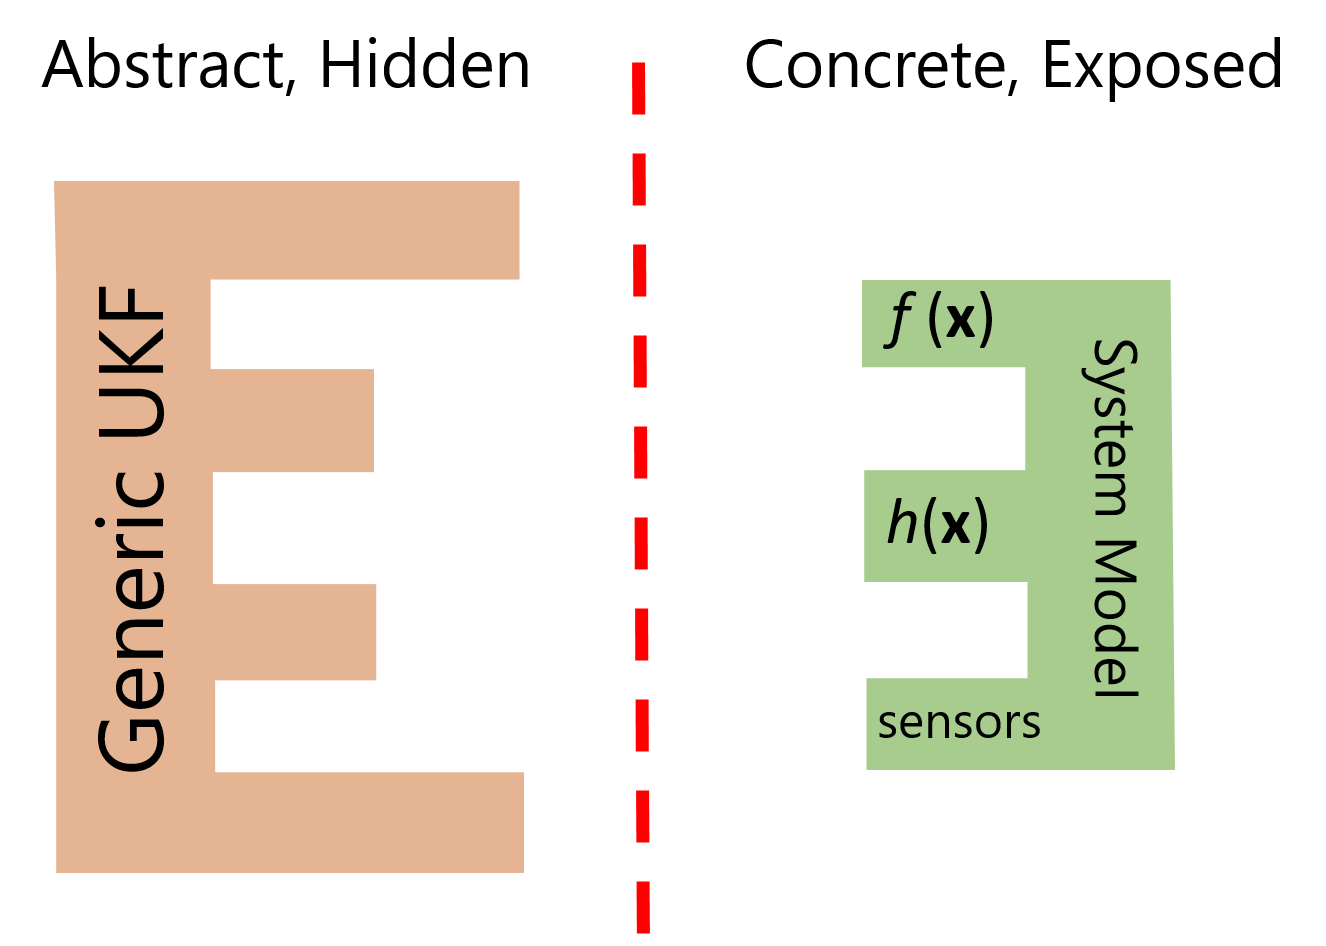
\includegraphics[width=0.5\textwidth]{generic_ukf}
        \caption[UKF Software Design]{A conceptual drawing of the underlying software design. The UKF algorithm is broken into a generic abstract class and a concrete subclass encoding vehicle specifics.}
        \label{fig:generic_ukf}
\end{figure}

The \texttt{UnscentedKf} class encapsulates the generic mathematics of the UKF without knowledge of particular system constraints. This class does little other than matrix mathematics and is designed to take as input the number of a system's states $n$ and its number of sensors $m$. With this information, \texttt{UnscentedKf} is able to populate a set of mean and covariance weights and then intelligently perform all of the requisite linear algebra for the UKF formulation. All other knowledge of particular states, sensors, vehicle geometry, and other metrics is hidden within subclasses such as \texttt{QuadUkf}.

\texttt{UnscentedKf} behaves in a manner similar to a Java interface in that it requires the extending class to supply functions codifying a process model and an observation model for the system under scrutiny. These two functions, along with $n$ and $m$, form the entirety of what \texttt{UnscentedKf} ``knows'' about the vehicle. All other details, including the fact that the class is being used in a ROS environment, are hidden from \texttt{UnscentedKf}. Because of this encapsulation of system specifics, the \texttt{UnscentedKf} class could be considered \textit{system agnostic}. This class implements only the bare-minimum functionality required for the Unscented Kalman Filter, and could thus be extended to any number of other systems, such as spacecraft, undersea vehicles, or automobiles. It is worth noting that \texttt{UnscentedKf}'s only software dependency is on the Eigen C++ linear algebra library\footnote{\url{www.eigen.tuxfamily.org}}, making it largely portable between operating systems.

The subclass (\texttt{QuadUkf} for the remainder of this thesis) handles all of the ROS communications for the given system. Specifically, this class has callback functions for receiving sensor data and is responsible for publishing state and covariance estimates. Figure~\ref{fig:data_flow} summarizes the data flow within the system. Upon arrival of an IMU message, the IMU callback function is triggered and the prediction step of the UKF is set in motion. When the system receives a pose message, the pose callback function is triggered and the correction step is set in motion. After every prediction and correction, a new belief is published and the system waits for further sensor data.

\begin{figure}
  \centering
    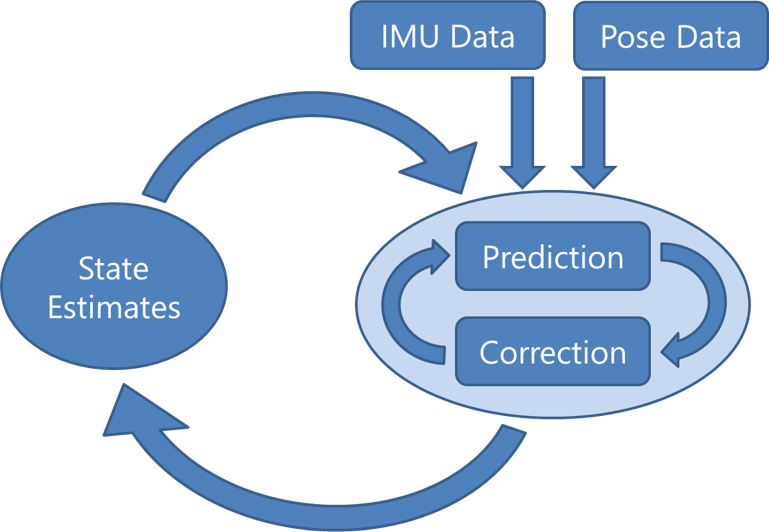
\includegraphics[width=0.6\textwidth]{data_flow}
  \caption[Data Flow Diagram]{Data flow within the system. The arrival of IMU and pose messages triggers the callback functions which predict and correct the estimated state of the system. After each prediction or correction, a new state estimate is published and the system waits for new sensor data.}
  \label{fig:data_flow}
\end{figure}
